\documentclass[12pt,a4paper]{article}

% ─── Encodage et langue ────────────────────────────────────────────────────
\usepackage[french]{babel}
\usepackage{newtxtext,newtxmath}
% ─── Mise en page ──────────────────────────────────────────────────────────
\usepackage[top=2.5cm, bottom=2.5cm, left=3cm, right=2.5cm]{geometry}
\usepackage{setspace}
\onehalfspacing

% ─── Titres de sections ────────────────────────────────────────────────────
\usepackage{titlesec}
\titleformat{\section}{\large\bfseries}{}{0em}{\thesection\quad}
\titleformat{\subsection}{\normalsize\bfseries}{}{0em}{\thesubsection\quad}

% ─── Tables ────────────────────────────────────────────────────────────────
\usepackage{booktabs}
\usepackage{array}
\usepackage{tabularx}

% ─── Graphiques ───────────────────────────────────────────────────────────
\usepackage{graphicx}

% ─── Couleurs et boîtes ────────────────────────────────────────────────────
\definecolor{rougeCMR}{RGB}{200, 16, 46}
\usepackage{xcolor}
\usepackage{mdframed}
\definecolor{bleuCMR}{RGB}{0, 62, 126}
\definecolor{vertCMR}{RGB}{0, 130, 60}
\definecolor{grisLight}{RGB}{245, 245, 245}

\mdfdefinestyle{encadre}{
  backgroundcolor=grisLight,
  linecolor=bleuCMR,
  linewidth=1pt,
  innertopmargin=8pt,
  innerbottommargin=8pt,
  innerleftmargin=10pt,
  innerrightmargin=10pt,
  roundcorner=4pt
}

% ─── Code source ───────────────────────────────────────────────────────────
\usepackage{listings}
\lstset{
  basicstyle=\ttfamily\small,
  backgroundcolor=\color{grisLight},
  frame=single,
  rulecolor=\color{bleuCMR!40},
  breaklines=true,
  showstringspaces=false,
  tabsize=4
}

% ─── Liens ─────────────────────────────────────────────────────────────────
\usepackage[hidelinks]{hyperref}

% ─── En-tête / pied de page ────────────────────────────────────────────────
\usepackage{fancyhdr}
\pagestyle{fancy}
\fancyhf{}
\fancyhead[L]{\small\textcolor{bleuCMR}{Simulation de pannes — Hôpital camerounais}}
\fancyhead[R]{\small\textcolor{bleuCMR}{\thepage}}
\renewcommand{\headrulewidth}{0.4pt}

% ══════════════════════════════════════════════════════════════════════════════
\begin{document}
% ══════════════════════════════════════════════════════════════════════════════

% ─── Page de titre ─────────────────────────────────────────────────────────
\begin{titlepage}
  \centering
  \vspace*{1.5cm}

  {\color{bleuCMR}\rule{\linewidth}{2pt}}
  \vspace{0.4cm}

  {\LARGE\bfseries Dispositif de prédiction de pannes d'électricité\\
  et de basculement automatique}

  \vspace{0.3cm}
  {\color{bleuCMR}\rule{\linewidth}{0.8pt}}

  \vspace{1cm}
  {\large\bfseries Rapport technique — Phase~1}\\
  \vspace{0.3cm}
  {\large Simulation de capteurs pour un hôpital camerounais\\
  avec ROS~2 Jazzy}

  \vspace{2cm}

  \begin{mdframed}[style=encadre]
    \centering
    \textbf{Environnement cible :} Hôpital $\sim$100~lits, Cameroun\\
    \textbf{Réseau simulé :} BTA 220~V / 50~Hz (Règlement MINEE, art.~14)\\
    \textbf{Outil de simulation :} ROS~2 Jazzy (Python)\\
    \textbf{Données de référence :} Moukengué Imano A.,
    Université de Douala, 2015
  \end{mdframed}

  \vfill
  {\small\today}
\end{titlepage}

% ─── Table des matières ────────────────────────────────────────────────────
\tableofcontents
\newpage

% ══════════════════════════════════════════════════════════════════════════════
\section{Fidélité à la description initiale du projet}
% ══════════════════════════════════════════════════════════════════════════════

Le projet repose sur deux objectifs formulés dans le cahier des charges~:
premièrement, déployer des \textbf{sondes} pour collecter des données
de pannes électriques dans un environnement cible~; deuxièmement,
construire un \textbf{modèle de prévision} capable de gérer automatiquement
le basculement entre la source principale et une source secondaire.

\subsection{Le déploiement des sondes}

Nous avons choisi d'implémenter les sondes sous la forme de
\textbf{nœuds Publishers ROS~2}, qui simulent des capteurs physiques
mesurant en continu~:

\begin{itemize}
  \item la \textbf{tension efficace} du réseau (Volts),
  \item la \textbf{fréquence} (Hertz),
  \item la \textbf{puissance active} consommée par l'hôpital (Watts),
  \item le \textbf{taux de distorsion harmonique} -- THD (\%),
  \item l'\textbf{état de coupure} et de \textbf{microcoupure} (booléen).
\end{itemize}

Cette approche satisfait pleinement le premier objectif~: la «~nature
diverse~» des capteurs est respectée par la multiplicité des grandeurs
mesurées, chacune publiée sur un canal ROS~2 indépendant.

\subsection{La collecte automatique vers un fichier structuré}

Un nœud Subscriber dédié (\texttt{data\_collector}) agrège en temps réel
tous les messages et les écrit dans un fichier CSV horodaté.
Ce fichier constitue le dataset d'entraînement du futur modèle ML,
conformément au second objectif du projet.

\subsection{La préparation du modèle de prédiction}

Toutes les colonnes du CSV ont été définies en vue d'un modèle de
classification binaire~: la colonne \texttt{outage} (0/1) est la
\textbf{variable à prédire}, et les autres colonnes sont les
\textbf{features d'entrée}. Ce lien est documenté en détail
à la section~\ref{sec:features}.

% ══════════════════════════════════════════════════════════════════════════════
\section{Architecture mise en place}
\label{sec:architecture}
% ══════════════════════════════════════════════════════════════════════════════

\subsection{Principe général de ROS~2}

ROS~2 (Robot Operating System~2) est un \textbf{intergiciel de communication}
entre programmes. Il joue le rôle de bus de messages~: les programmes ne
se parlent pas directement~; ils déposent des messages sur des canaux
nommés appelés \textbf{Topics}, et d'autres programmes les récupèrent.

Il ne mesure rien physiquement~; c'est le code Python qui génère
(ou, en production, lit sur un vrai capteur) les valeurs numériques,
les emballe dans un message ROS~2 typé, et les injecte dans le Topic.
Remplacer le simulateur par un capteur réel ne nécessitera aucune
modification du collecteur ni du modèle.

\subsection{Les quatre couches du pipeline}

\begin{center}
\begin{tabular}{p{0.05\linewidth} p{0.25\linewidth} p{0.55\linewidth}}
\toprule
\textbf{\#} & \textbf{Couche} & \textbf{Rôle} \\
\midrule
1 & Publisher (capteur) &
  Génère et publie les données électriques simulées toutes les 2~s. \\
2 & Topics ROS~2 &
  Bus de messages nommés (\texttt{/electricity/voltage}, etc.)~;
  découplent le producteur du consommateur. \\
3 & Subscriber (collecteur) &
  Reçoit chaque message, calcule les features dérivées, écrit le CSV. \\
4 & Fichier CSV &
  Dataset brut prêt pour scikit-learn / pandas. \\
\bottomrule
\end{tabular}
\end{center}

\subsection{Topics publiés}

\begin{center}
\begin{tabular}{p{0.38\linewidth} p{0.15\linewidth} p{0.35\linewidth}}
\toprule
\textbf{Topic} & \textbf{Type} & \textbf{Description} \\
\midrule
\texttt{/electricity/voltage}      & \texttt{Float32} & Tension efficace (V) \\
\texttt{/electricity/frequency}    & \texttt{Float32} & Fréquence (Hz) \\
\texttt{/electricity/power}        & \texttt{Float32} & Puissance active (W) \\
\texttt{/electricity/thd}          & \texttt{Float32} & Distorsion harmonique (\%) \\
\texttt{/electricity/outage}       & \texttt{Bool}    & Coupure complète \\
\texttt{/electricity/micro\_outage} & \texttt{Bool}   & Microcoupure (\textless~10~s) \\
\texttt{/electricity/raw\_data}    & \texttt{String}  & JSON complet (toutes mesures) \\
\bottomrule
\end{tabular}
\end{center}
\clearpage
\subsection{Schéma du circuit mis en place}
\begin{figure}[htbp]
  \centering
  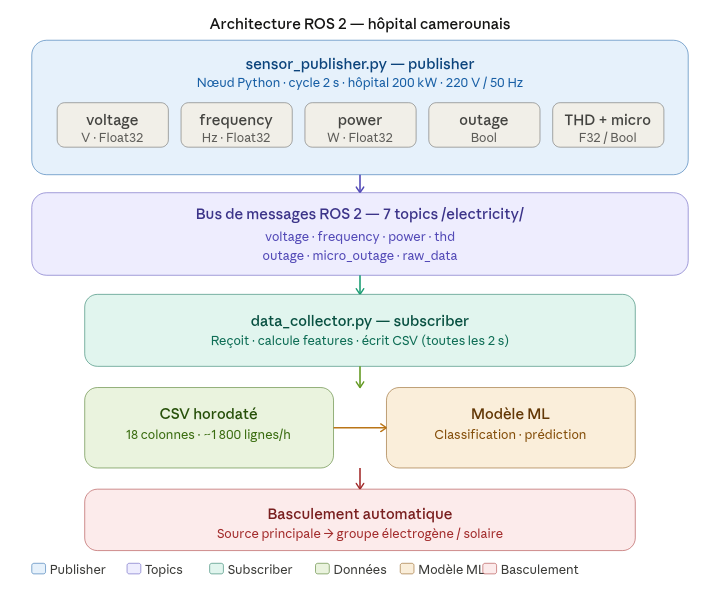
\includegraphics[width=0.8\textwidth]{circuit_diagram.png}
  \caption{Pipeline ROS\textasciitilde{}2~: flux de données du Publisher au CSV.}
  \label{fig:circuit}
\end{figure}

% ══════════════════════════════════════════════════════════════════════════════
\section{Adaptation du code au contexte camerounais\\
selon le manuscrit de référence}
\label{sec:manuscrit}
% ══════════════════════════════════════════════════════════════════════════════

L'adaptation s'appuie sur les mesures réelles publiées par
\textbf{Moukengué Imano}~\cite{moukengue2015}~: enregistrements
chronologiques effectués en août~2015 dans des installations BTA
du quartier Ndogbong, Douala.

\subsection{Paramètres légaux de référence}

L'article~14 du Règlement du Service de distribution publique d'électricité
du Cameroun (Arrêté MINEE n°~00000013, 26~janvier~2009) fixe~:

\begin{mdframed}[style=encadre]
\begin{itemize}
  \item Tension nominale~: \textbf{220/380~V}, tolérance \textbf{$\pm$10\,\%}
    (plage légale~: 198~V -- 242~V)
  \item Fréquence nominale~: \textbf{50~Hz}, tolérance \textbf{$\pm$5\,\%}
    (plage légale~: 47,5~Hz -- 52,5~Hz)
\end{itemize}
\end{mdframed}

\subsection{Paramètres numériques corrigés}

\begin{center}
\begin{tabularx}{\linewidth}{p{0.28\linewidth} p{0.22\linewidth}
                              p{0.22\linewidth} p{0.18\linewidth}}
\toprule
\textbf{Paramètre} & \textbf{Ancien code} & \textbf{Nouveau code}
                   & \textbf{Source} \\
\midrule
Puissance nominale &
  2~000~W (foyer) & 200~000~W (hôpital) & §3.4 manuscrit \\
Bruit tension -- jour &
  $\mathcal{N}(0,\;8)$ &
  $\mathcal{N}(-6{,}6,\;13)$ &
  Tableau~1 \\
Bruit tension -- nuit &
  $\mathcal{N}(0,\;8)$ &
  $\mathcal{N}(0{,}6,\;10)$ + pics &
  Tableau~1 \\
Bruit fréquence -- jour &
  $\mathcal{N}(0,\;0{,}5)$ &
  $\mathcal{N}(51{,}75,\;2{,}3)$ + pics &
  Tableau~2 \\
Proba. coupure &
  2\,\% uniforme &
  1--5\,\% selon heure &
  §3.4 manuscrit \\
Profil de charge &
  Sinusoïde résidentielle &
  Profil hôpital 45--100\,\% &
  §3.4 manuscrit \\
\bottomrule
\end{tabularx}
\end{center}

Les valeurs mesurées dans le Tableau~1 du manuscrit montrent
une tension pouvant descendre à \textbf{205,5~V} en journée et
monter jusqu'à \textbf{260,2~V} la nuit~-- deux cas hors tolérance légale
reproduits dans la simulation.

Le Tableau~2 révèle une fréquence maximale mesurée de \textbf{66,21~Hz}
lors d'une journée ouvrable, soit un écart de $+$16,21~Hz par rapport
au nominal, très au-delà de la tolérance de $\pm$5\,\%.
Ces pics sont simulés avec une probabilité de~3\,\% par cycle de jour.

% ══════════════════════════════════════════════════════════════════════════════
\section{Types de pannes simulées}
\label{sec:pannes}
% ══════════════════════════════════════════════════════════════════════════════

Le code v2.0 simule \textbf{quatre types de dysfonctionnements},
chacun documenté dans le manuscrit de référence.

\subsection{Coupure complète (\emph{outage})}

\begin{mdframed}[style=encadre]
\textbf{Définition~:} interruption totale de l'alimentation (tension = 0~V,
fréquence = 0~Hz, puissance = 0~W).\\
\textbf{Durée simulée~:} de 1~minute à 6~heures (distribution uniforme).\\
\textbf{Probabilité~:} variable selon l'heure -- 1\,\% la nuit,
2,5\,\% en journée, 5\,\% en heure de pointe (18h--22h).\\
\textbf{Signal précurseur~:} chute progressive de tension dans les cycles
qui précèdent la coupure, reproduisant les creux de tension décrits
au §3.3.1 du manuscrit.\\
\textbf{Variable CSV~:} \texttt{outage} = 1.
\end{mdframed}

\subsection{Microcoupure (\emph{micro\_outage})}

\begin{mdframed}[style=encadre]
\textbf{Définition~:} interruption brève de 2~à~10~secondes,
indépendante de la coupure complète.\\
\textbf{Cause dans le manuscrit (§4.2)~:} démarrage direct simultané
de gros moteurs (menuiseries, machines de quartier), postes de soudure.
Le manuscrit précise qu'elles sont \og{}plus dangereuses que les coupures
prolongées\fg{} pour le matériel électronique médical.\\
\textbf{Probabilité~:} 4\,\% par cycle.\\
\textbf{Variable CSV~:} \texttt{micro\_outage} = 1.
\end{mdframed}

\subsection{Tension hors tolérance légale}

\begin{mdframed}[style=encadre]
\textbf{Définition~:} tension efficace en dehors de la plage 198--242~V
($\pm$10\,\% autour de 220~V).\\
\textbf{Cas observés dans le manuscrit (Tableau~1)~:} survoltage
nocturne mesuré à 260,2~V~; dévoltage en journée à 205,5~V,
causés par la surcharge des transformateurs et les installations
non conformes.\\
\textbf{Variable CSV~:} \texttt{voltage\_out\_of\_tolerance} = 1.
\end{mdframed}

\subsection{Fréquence hors tolérance légale}

\begin{mdframed}[style=encadre]
\textbf{Définition~:} fréquence en dehors de la plage 47,5--52,5~Hz
($\pm$5\,\% autour de 50~Hz).\\
\textbf{Cas observés dans le manuscrit (Tableau~2)~:} fréquence maximale
mesurée de 66,21~Hz en journée et de 67,20~Hz la nuit.
Ces anomalies sont liées aux équipements polluants raccordés en BTA
(pollution harmonique).\\
\textbf{Variable CSV~:} \texttt{freq\_out\_of\_tolerance} = 1.
\end{mdframed}

\subsection{Distorsion harmonique (THD) élevée}

\begin{mdframed}[style=encadre]
\textbf{Définition~:} taux de distorsion harmonique supérieur à 5\,\%
(norme acceptable). La simulation produit des valeurs entre 8 et 20\,\%.\\
\textbf{Cause dans le manuscrit (§3.4)~:} lampes économiques bas de gamme,
alimentations à découpage des équipements médicaux (moniteurs, IRM).
Le manuscrit identifie ce phénomène comme un \og{}nouveau problème
de pollution harmonique dans les quartiers\fg{}.\\
\textbf{Variable CSV~:} \texttt{thd\_percent}.
\end{mdframed}

% ══════════════════════════════════════════════════════════════════════════════
\section{Features du modèle de prédiction}
\label{sec:features}
% ══════════════════════════════════════════════════════════════════════════════

\subsection{Qu'est-ce qu'une feature~?}

\begin{mdframed}[style=encadre]
Une \textbf{feature} (ou \emph{variable d'entrée}) est une information
numérique mesurable que l'on fournit au modèle de Machine Learning
pour qu'il puisse apprendre.

\medskip
\noindent
\textbf{Analogie~:} pour prédire si une personne est malade, on donne
au médecin sa température, sa tension artérielle, et son âge.
Ces trois valeurs sont les \emph{features}. La réponse
\og{}malade ou non\fg{} est la \emph{variable cible}.

\medskip
\noindent
Dans notre projet~: les mesures électriques (tension, fréquence,
THD, etc.) sont les \emph{features}. La coupure imminente (oui/non)
est la \emph{variable cible} que le modèle doit apprendre à prédire
\textbf{avant} qu'elle ne survienne.
\end{mdframed}

\subsection{Variable cible (ce que le modèle doit prédire)}

\begin{center}
\begin{tabular}{p{0.3\linewidth} p{0.12\linewidth} p{0.45\linewidth}}
\toprule
\textbf{Colonne CSV} & \textbf{Valeurs} & \textbf{Signification} \\
\midrule
\texttt{outage}      & 0 ou 1 &
  Coupure complète en cours~: c'est la \textbf{cible principale}.
  Le modèle doit la prédire quelques cycles à l'avance. \\
\texttt{micro\_outage} & 0 ou 1 &
  Microcoupure~: cible secondaire pour un modèle de détection fine. \\
\bottomrule
\end{tabular}
\end{center}

\subsection{Features d'entrée du modèle}

Les features sont regroupées en quatre catégories.

\bigskip
\noindent
\textbf{(a) Features de mesure brute} — ce que les capteurs lisent directement~:

\begin{center}
\begin{tabular}{p{0.32\linewidth} p{0.55\linewidth}}
\toprule
\textbf{Feature} & \textbf{Ce qu'elle apporte au modèle} \\
\midrule
\texttt{voltage\_v}     &
  Une tension qui chute en dessous de 198~V \emph{avant} la coupure
  est le signal le plus fort identifié dans le manuscrit. \\
\texttt{frequency\_hz}  &
  Une fréquence hors norme indique une surcharge ou un défaut réseau
  imminent. \\
\texttt{power\_w}       &
  Une chute soudaine de puissance peut précéder une coupure,
  même si la tension paraît encore acceptable. \\
\texttt{thd\_percent}   &
  Un THD qui monte brusquement signale une surcharge du transformateur,
  précurseur documenté de coupure (\S3.4 du manuscrit). \\
\bottomrule
\end{tabular}
\end{center}

\bigskip
\noindent
\textbf{(b) Features de conformité légale} — calculées à partir des mesures~:

\begin{center}
\begin{tabular}{p{0.38\linewidth} p{0.49\linewidth}}
\toprule
\textbf{Feature} & \textbf{Ce qu'elle apporte au modèle} \\
\midrule
\texttt{voltage\_deviation}          &
  Écart en Volts par rapport à 220~V. Une valeur négative croissante
  est un signal précurseur de coupure. \\
\texttt{freq\_deviation}             &
  Écart en Hz par rapport à 50~Hz. \\
\texttt{voltage\_out\_of\_tolerance} &
  Indicateur binaire 0/1~: la tension dépasse-t-elle les limites
  légales~? Enrichit le modèle avec un signal discret. \\
\texttt{freq\_out\_of\_tolerance}    &
  Idem pour la fréquence. \\
\bottomrule
\end{tabular}
\end{center}

\bigskip
\noindent
\textbf{(c) Features temporelles} — le moment de la mesure~:

\begin{center}
\begin{tabular}{p{0.38\linewidth} p{0.49\linewidth}}
\toprule
\textbf{Feature} & \textbf{Ce qu'elle apporte au modèle} \\
\midrule
\texttt{hour}         &
  Heure locale (0--23). La probabilité de coupure varie fortement
  selon l'heure (pointe 18h--22h vs nuit). \\
\texttt{is\_peak\_hour} &
  Binaire~: 1 si l'heure est en période de pointe (18h--22h),
  période de surcharge maximale du réseau. \\
\texttt{is\_night}    &
  Binaire~: 1 si l'heure est nocturne (22h--6h), période de
  survoltage documenté dans le manuscrit. \\
\bottomrule
\end{tabular}
\end{center}

\bigskip
\noindent
\textbf{(d) Features historiques} — la mémoire du système~:

\begin{center}
\begin{tabular}{p{0.38\linewidth} p{0.49\linewidth}}
\toprule
\textbf{Feature} & \textbf{Ce qu'elle apporte au modèle} \\
\midrule
\texttt{cycles\_since\_last\_outage} &
  Nombre de cycles sans coupure. Un réseau \og{}calme depuis longtemps\fg{}
  tend à accumuler les contraintes~; cette feature capture ce phénomène
  de \emph{fatigue réseau}. \\
\texttt{outage\_count}        &
  Nombre total de coupures depuis le démarrage.
  Caractérise la fiabilité globale du réseau sur la session. \\
\texttt{micro\_outage\_count} &
  Nombre total de microcoupures.
  Une fréquence élevée de microcoupures précède souvent
  une coupure franche. \\
\bottomrule
\end{tabular}
\end{center}

\subsection{Récapitulatif du CSV}

Le fichier CSV produit par la simulation comporte
\textbf{18~colonnes} et \textbf{une ligne toutes les 2~secondes},
soit environ 1~800~lignes par heure de simulation.

\begin{center}
\begin{tabular}{lcc}
\toprule
\textbf{Catégorie} & \textbf{Colonnes} & \textbf{Rôle ML} \\
\midrule
Identification      & 2  & (hors modèle) \\
Mesures brutes      & 4  & Features \\
Variables cibles    & 2  & Labels \\
Conformité légale   & 4  & Features \\
Temporelles         & 3  & Features \\
Historiques         & 3  & Features \\
\midrule
\textbf{Total}      & \textbf{18} & \textbf{14 features + 2 labels} \\
\bottomrule
\end{tabular}
\end{center}

% ══════════════════════════════════════════════════════════════════════════════
\section*{Conclusion}
\addcontentsline{toc}{section}{Conclusion}
% ══════════════════════════════════════════════════════════════════════════════

La simulation développée est \textbf{fidèle à la description initiale du projet}
sur les deux objectifs~: les sondes sont déployées (sous forme de nœuds
ROS~2 Publishers) et les données sont collectées dans un format directement
exploitable par un modèle de Machine Learning.

Elle est également \textbf{ancrée dans la réalité camerounaise} grâce aux
mesures publiées par Moukengué Imano~: les distributions statistiques de
tension et de fréquence, les profils horaires de charge, et les probabilités
de coupure reproduisent fidèlement les conditions du réseau BTA à Douala.

La prochaine étape est l'entraînement d'un modèle de classification
(Random Forest, LSTM ou gradient boosting) sur ce dataset, avec
\texttt{outage} comme variable cible et les 14~features comme entrées.

% ─── Références ────────────────────────────────────────────────────────────
\begin{thebibliography}{9}

\bibitem{moukengue2015}
  Moukengué Imano~A.,
  \textit{Problèmes d'électrification urbaine au Cameroun~:
  diagnostic et proposition de solutions curatives},
  Équipe de Recherche en Systèmes d'Énergie Électrique,
  Laboratoire LEEAT, Université de Douala, Novembre~2015.

\bibitem{minee2009}
  Ministère de l'Énergie et de l'Eau du Cameroun,
  \textit{Arrêté n°~00000013/MINEE du 26~janvier~2009 portant approbation
  du Règlement du Service de distribution publique d'électricité},
  Yaoundé, 2009.

\bibitem{loi2011}
  République du Cameroun,
  \textit{Loi N°~2011/022 du 14~décembre~2011 régissant le secteur
  d'électricité au Cameroun},
  Assemblée Nationale, Yaoundé, 2011.

\end{thebibliography}

\end{document}
